\documentclass[12pt]{report}
\usepackage{sectsty}
\usepackage{parskip}
\usepackage{hyperref}
\usepackage{varwidth}
\usepackage[hypcap]{caption}
\usepackage[list=true]{subcaption}
\usepackage{tikz}
\usepackage{alltt}
\renewcommand{\Large}{\fontsize{18pt}{18pt}\selectfont}
\renewcommand{\large}{\fontsize{14pt}{14pt}\selectfont}
\sectionfont{\large}
\renewcommand{\thesection}{\arabic{section}}
\def\sectionautorefname{Section}
\usetikzlibrary{scopes}
\usetikzlibrary{chains}
\usetikzlibrary{shapes}
\usetikzlibrary{positioning}
\usetikzlibrary{fit}
\begin{document}

\begin{titlepage}
\vspace*{\fill}
\begin{center}
{\Large Obstacle Detection and Avoidance Using TurtleBot Platform and XBox Kinect} \\
\vspace{18pt}
{\large Sol Boucher} \\
\vspace{14pt}
{\large Research Assistantship Report \\
	Department of Computer Science \\
	Rochester Institute of Technology} \\
\vspace{14pt}
Research Supervisor: Dr. Roxanne Canosa \\
Research Sponsor: Golisano College Honors Committee \\
\vspace{12pt}
20114/\today
\end{center}
\vspace{\fill}
Roxanne Canosa, Ph.D. \hrulefill\ Date \hrulefill
\end{titlepage}

\begin{abstract}
\thispagestyle{plain}
\setcounter{page}{2}
Any robot that is to drive autonomously must be able to detect and avoid obstacles that it might encounter.  Traditionally, this problem has been solved using systems of one or more RGB cameras utilizing complicated and computationally-expensive computer vision algorithms, somewhat unreliable ultrasonic distance sensors, or laser-based depth scanners.  However, Microsoft's recent release of the XBox Kinect has opened up new areas of research in the areas of computer vision and image understanding, and this same device can be employed for obstacle detection. \\
The three-dimensional point cloud provided by the low-cost and commercially-available Kinect platform puts much more information about the surrounding world at the disposal of an autonomous robot.  This research investigates the problem of using this data to autonomously detect and avoid obstacles in an unconstrained indoor environment.  The algorithm used is a synthesis of the traditional method of choosing turn directions based on the centroid of the detected points and a  more novel search of the ground plane for edges and boundaries.  Good results are achieved not only for drop-offs and common obstructions, but also when objects are especially short or moving just in front of the robot and perpendicular to it.
\end{abstract}

\setcounter{page}{3}
\tableofcontents
\clearpage
\phantomsection
\addcontentsline{toc}{section}{List of Figures}
\listoffigures
\clearpage
\phantomsection
\addcontentsline{toc}{section}{List of Tables}
\listoftables
\newpage

\section{Introduction}
This research was conducted on Willow Garage's TurtleBot robotics platform, an integrated kit backed by their ROS robotics suite and the Open Perception Foundation's Point Cloud Library.  The goal was to implement a simple but effective obstacle detection and avoidance system that---using only the data from the Kinect---was able to autonomously roam the hallways on all floors of the building without running into anything.  This task presupposed an ability to avoid whatever common hazards, whether stationary or mobile, it might reasonably be expected to encounter during such a journey.  Such capability would be desirable for potential use with or integration into future projects developed on the same system or a similar one.

\section{Similar Work (Literature Review)}
The XBox Kinect has an infrared projector and infrared camera separated by about 7.5 cm, and a color camera about 2 cm away from the latter.  The infrared pair is able to assemble a grid of distance measurements triangulated from the lateral displacement of the projected points from the known emitter pattern.  Unfortunately, the device is unable to perform any distance measurements closer than about 0.5 m.  One method of detecting obstacles is as follows:  First, perform a voxel grid downsampling on the point cloud to decrease processing time.  Next, apply a pass-through filter to crop out regions of little interest or accuracy.  Then, use the RANSAC algorithm to perform plane detection.  Finally, Euclidean cluster extraction reveals individual obstacles, and additional analysis of those obstacles is performed in order to determine their sizes.  This procedure avoids many difficulties of using a single RGB camera, as well as enjoying faster run times than dual--RGB camera systems (\hyperref[bib:nguyen]{Nguyen, 2012}).

Whenever information from multiple image sensors is integrated, there is a risk that it will not line up appropriately, either due to simple displacement resulting from the sensors' relative positions or because of unique lens distortions created by inconsistencies in the manufacturing process.  Herrera \textit{et al.} describe their noise-tolerant method for calibrating a color camera and depth camera against each other, enabling the attainment of better results than would ever be possible by calibrating the two cameras individually.  They start by computing for the color camera the two-dimensional projection coordinates in the image at which a three-dimensional point in space---the corner of a checkerboard calibration pattern---appears, then perform a distortion correction.  Next, they repeat the projection calculation for the depth image, this time using the corners of the plane on which the checkerboard rests---because the board itself isn't visible in this image---and omitting the distortion correction step, as it will be much less effective than for the color imagery.  Using the projections and data from several images with different perspectives, it is possible to calculate the rotation and translation necessary to match the two images' reference frames.  These first parameters obtained for the color camera are much better than those for the depth sensor, so the former are used to optimize the latter by performing a nonlinear error minimization; then, another minimization is performed across the parameters for both cameras until the results are convergent.  Using 35 calibration images, the authors are able to demonstrate comparable accuracy to that achieved by the proprietary calibration algorithm provided with their XBox Kinect test sensor (\hyperref[bib:herrera]{Herrera \textit{et al.}, 2011}).

A common traditional method of obstacle avoidance is the potential field model, or PFM.  This model represents targets and obstacles as imaginary attractive and repulsive forces on the robot, respectively.  Stored as vectors, such forces are easily summed to find the resultant force vector, which is used directly as the robot's navigation vector.  One such implementation---the virtual force field, or VFF---uses a two-dimensional histogram grid populated from ultrasonic range sensors and holding certainty values of how likely it is that an obstacle exists at each location.  Objects of interest are assigned corresponding virtual repulsive force vectors with magnitude proportional to their certainty values and inversely proportional to their distance from the vehicle's center.  Similarly, the attractive force between the robot and its goal location is proportional to a preassigned force constant and inversely proportional it its distance from the vehicle.  After obtaining the resultant force vector, its direction and magnitude are converted into parameters usable by the drive system and issued as movement commands.  However, four major problems have been identified that effect all PFM systems, becoming increasingly noticeable as a robot moves faster:  The robot may fall into a trap situation when it reaches a dead end, a phenomenon for which workarounds exist.  The robot may also be directed in the opposite direction of its target in the case where two close objects stand in front of it with space between, a more difficult problem to handle.  Certain environments may also cause the robot to begin oscillating.  Finally, more severe oscillations---and even collisions---occur when a robot drives down a narrow hallway with a discontinuity in its side.  Together, these factors make the same PFMs that were once seen as simple and elegant much less attractive, especially for applications relying on higher speeds (\hyperref[bib:koren]{Koren and Borenstein, 1999}).

One way to detect obstacles using an RGB-D camera is to segment every plane in the point cloud and consider as obstacles both points emerging from the detected planes and planes whose surface orientations differ from that of the ground.  Surface detection may be accomplished computationally cheaply by considering pixel neighborhoods instead of performing distance searches, then computing the normal vector by finding the cross-product of two averaged vectors tangential to the local surface.  The coordinates of the points and their corresponding surface normals are transformed to Cartesian coordinates from the robot's perspective, then to spherical coordinates.  Only the plane representing the ground is considered navigable, and the RANSAC algorithm is applied to optimize the detected surfaces and compensate for noisy readings.  Each plane is then converted to its convex hull, and both horizontal planes other than the ground and planes supported by horizontal planes are considered to be navigational obstacles.  This method is able to process plane data at high speed using only sequential processing while remaining relatively accurate: the average deviation is under ten degrees, and objects are properly segmented over 90\% of the time.  The algorithm is, however, sensitive to very small objects and distant measurements (\hyperref[bib:holz]{Holz \textit{et al.,} 2011}).

Another method of making use of depth information for the purpose of detecting obstacles is to examine the 3-D slopes between detected points.  The points may be considered to compose a single obstacle if this slope---measured with respect to the horizontal---is steeper than a set slope and if their height difference falls within a predetermined range.  Such obstacles may be found by searching the image from the bottom row and finding for each obstacle pixel in that row all the other pixels that meet the aforementioned criteria with respect to that pixel.  The resulting points may also be classified as obstacle points, and the process repeated to find all such associated points.  Finally, individual objects may be picked out by applying the transitive property of the above obstacle composition criteria.  This works very well if the terrain and robot are both flat, but becomes a more difficult task as the terrain becomes rough or if the robot is expected to climb ramps (\hyperref[bib:talukder]{Talukder, 2002}).

Although the latter few approaches offer robust, proven functionality and are highly applicable to the type of sensor used, this project sought a simpler solution and didn't require segmentation or identification of individual objects.  Thus, it began instead with the development of what would evolve into an implementation of one of the most common simple obstacle avoidance algorithms, simply turning away from the centroid of the detected offending points.  However, this venerable approach was extended to consider not only obstacles themselves but also edges on the ground plane, an addition that enabled the detection of several additional danger scenarios that could not be handled by the traditional method alone.

\section{Background}
The Point Cloud Library includes many data types and numerous algorithms that make working with point clouds extraordinarily easy.  The first of the algorithms used in this research was the 3-D voxel grid filter, which downsamples point cloud data by modeling the input dataset with a three-dimensional grid having cubic cells of user-supplied dimensions.  Each cell containing at least one point in the original image is then populated with a single voxel placed at the centroid of the points within that part of the input (\hyperref[bib:rusu]{Rusu, 2011}).

The research also made extensive use of the plane edge detection algorithms simultaneously developed by Changhyun Choi, a Ph.D. student at the Georgia institute of technology.  One of the utilized algorithms simply finds points bordering on those whose coordinates are set to NaN values, thereby computing the absolute boundaries of a plane.  Particularly useful was his high curvature edge detection algorithm, which locates the points making up the boundaries between the floor and those objects that rest on it using integral images and Canny edge detection (\hyperref[bib:choi]{Choi, 2012}).

Integral images are a common technique in modern computer vision, and are used to detect distinctive image features.  They are essentially tables storing for each coordinate in the corresponding image the sum of the pixel values lying in the box bounded by that coordinate and the upper-left corner of the image.  Features from an integral image can then be used for a wide variety of purposes, including estimation of a 3-D image's surface normals (\hyperref[bib:viola]{Viola, 2001}).

The Canny edge detector starts by smoothing the input image to reduce noise.  Next, the spacial gradients of the resulting image are measured in order to expose the edges, each of which is assigned a strength based on the distinctiveness of its gradient.  The directions of the edges are determined in two dimensions using these gradients, then the directions are used to trace the edges.  Those edges with strengths above a certain threshold are kept, while those with strengths between that value and a lower constant are kept only if they are connected to one or more edges from the former group (\hyperref[bib:canny]{Canny, 1986}).

PCL also provides a radius outlier removal, which accepts from the user a search radius and a minimum number of neighbors.  It then searches the neighborhood surrounding each point in the image and removes that point if it has fewer than the specified number of neighbors (\hyperref[bib:oleary]{O'Leary, 2011}).

As the project progressed, it became necessary to discern information about the ground plane directly in front of the robot.  In order to determine which points were part of this plane, a linear model was calculated from the y- and z-coordinates of two known floor points, one---$(z_1,y_1)$---very near to the robot and the other---$(z_2,y_2)$---farther away.  First, the plane's slope $m$ was computed, as in \autoref{eq:slope}:
\begin{equation}
\label{eq:slope}
m=\frac{y_2-y_1}{z_2-z_1}
\end{equation}
Next, the y-intercept $y_0$ was calculated using the average of the coordinates substituted into the point-slope form of a linear equation (\autoref{eq:intercept}):
\begin{equation}
\label{eq:intercept}
y_0=\frac{y_1+y_2}{2}-m\frac{z_1+z_2}{2}
\end{equation}
The resulting slope and intercept were both stored; thus, the y-coordinate corresponding to a given z-coordinate could be calculated using \autoref{eq:line}'s simple linear equation:
\begin{equation}
\label{eq:line}
y=mz+y_0
\end{equation}
Sufficient deviation of the z-coordinate from its expected value allowed the conclusion that the point was not, in fact, part of the ground.  Another---slightly less strict---threshold was used to broaden consideration to points that were very near the ground plane, as well as those actually composing it.

\section{Approach}
\label{sec:approach}
\begin{figure}
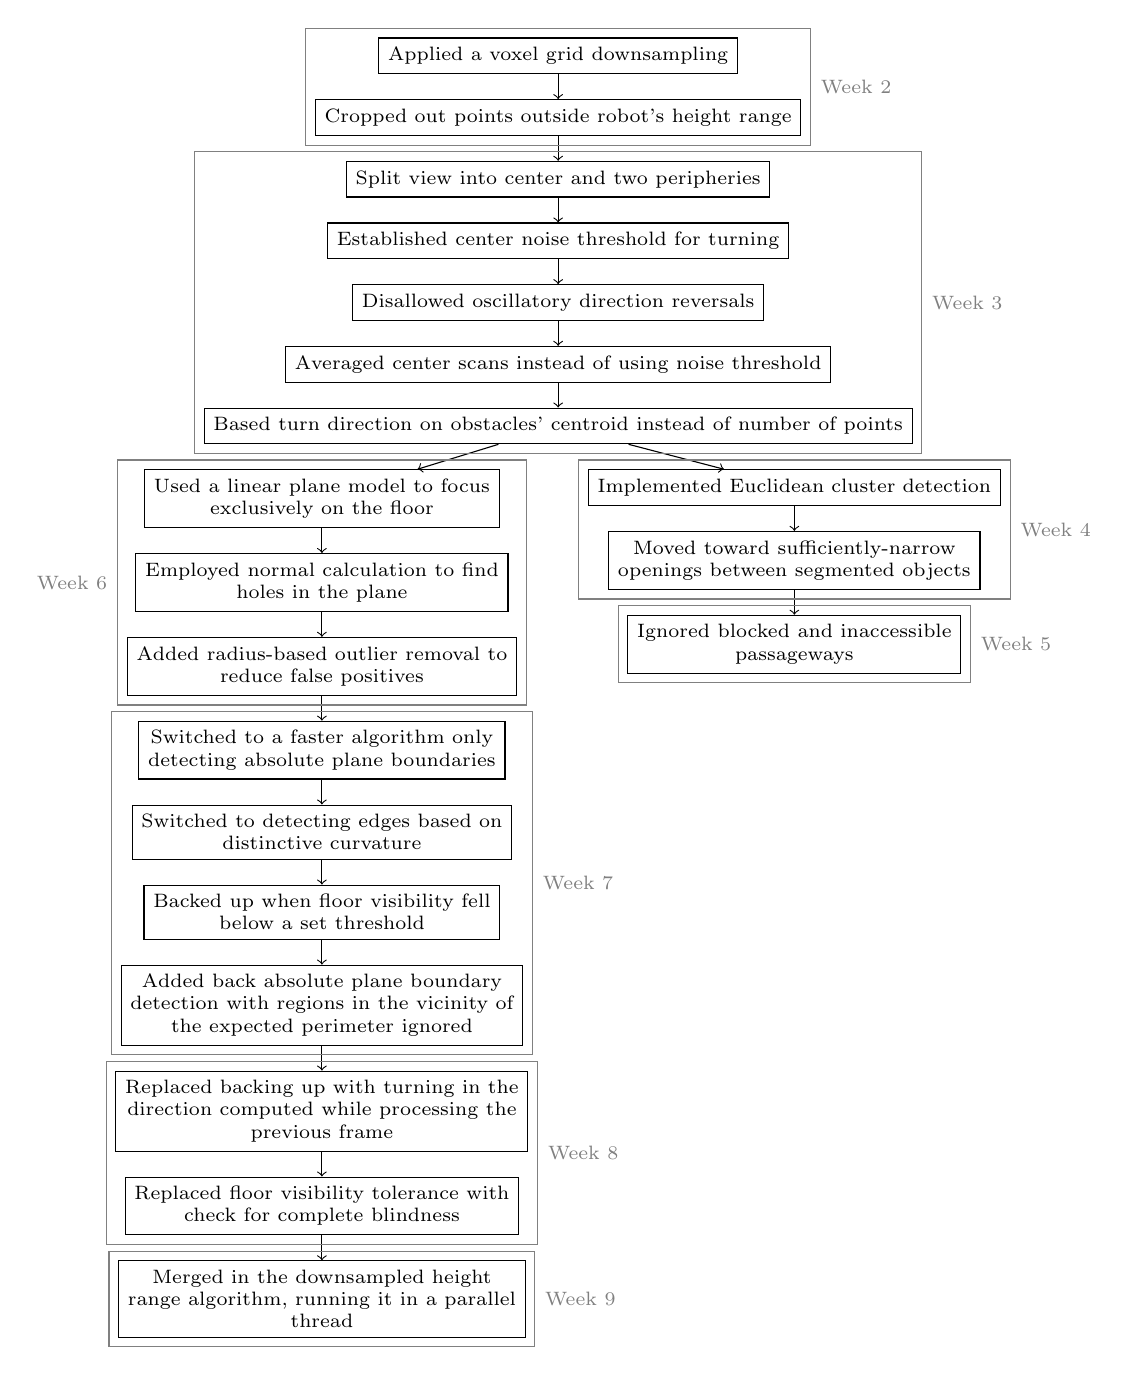
\begin{tikzpicture}[start chain=going below, every node/.style={draw,on chain,font=\scriptsize}, every on chain/.style=join, every join/.style=->, node distance=9pt]
\node{Applied a voxel grid downsampling};
\node{Cropped out points outside robot's height range};
\node{Split view into center and two peripheries};
\node{Established center noise threshold for turning};
\node{Disallowed oscillatory direction reversals};
\node{Averaged center scans instead of using noise threshold};
\node{Based turn direction on obstacles' centroid instead of number of points};
{ [every node/.append style={execute at begin node={\begin{varwidth}{5cm}\begin{center}},execute at end node={\end{center}\end{varwidth}}}]
	{ [start branch=cluster-detect going below]
		\node[xshift=3cm]{Implemented Euclidean cluster detection};
		\node{Moved toward sufficiently-narrow openings between segmented objects};
		\node{Ignored blocked and inaccessible passageways};
	}
	\node[xshift=-3cm]{Used a linear plane model to focus exclusively on the floor};
	\node{Employed normal calculation to find holes in the plane};
	\node{Added radius-based outlier removal to reduce false positives};
	\node{Switched to a faster algorithm only detecting absolute plane boundaries};
	\node{Switched to detecting edges based on distinctive curvature};
	\node{Backed up when floor visibility fell below a set threshold};
	\node{Added back absolute plane boundary detection with regions in the vicinity of the expected perimeter ignored};
	\node{Replaced backing up with turning in the direction computed while processing the previous frame};
	\node{Replaced floor visibility tolerance with check for complete blindness};
	\node{Merged in the downsampled height range algorithm, running it in a parallel thread};
}
{ [color=gray, every node/.style={draw,font=\scriptsize}]
    \node[fit=(chain-1)(chain-2),label=right:Week 2]{};
    \node[fit=(chain-3)(chain-7),label=right:Week 3]{};
    \node[fit=(chain/cluster-detect-2)(chain/cluster-detect-3),label=right:Week 4]{};
    \node[fit=(chain/cluster-detect-4),label=right:Week 5]{};
    \node[fit=(chain-8)(chain-10),label=left:Week 6]{};
    \node[fit=(chain-11)(chain-14),label=right:Week 7]{};
    \node[fit=(chain-15)(chain-16),label=right:Week 8]{};
    \node[fit=(chain-17),label=right:Week 9]{};
}
\end{tikzpicture}
\caption{The progression of code development}
\label{fig:progression}
\end{figure}

The point cloud coming off the Kinect exhibited noticeable noise, was extremely dense, and was consequently slow to transmit, display, and process.  Thus, the first action taken was the application of a voxel grid filter to downsample the data and eradicate most of the noise while achieving better update speeds and faster processing time.  Noticing that both Holz \textit{et al.} and Nguyen used surface detection algorithms, while Koren and Borenstein simply didn't train sensors on the floor, a decision was made to crop the y-dimension so as to discard all points falling outside the robot's height range.  This step---which was possible because the robot was going to be used chiefly in indoor environments possessing smooth terrain---made it possible to ignore the floor and focus exclusively on those points that represented actual obstacles.  However, it also meant sacrificing the ability to climb ramps and traverse highly uneven floors.

The initial revision of the obstacle avoidance algorithm simply split the view into three parts:  The center region was used to determine whether to proceed forward or turn, the latter of which was triggered whenever the number of points in this region exceeded a set noise threshold.  Once the robot had entered a turning mode, it ceased forward motion and decided on a direction by choosing the peripheral vision field with fewer points in it.  The entire field of view was cropped in the z-dimension in order to prevent the robot from being distracted by objects well ahead of its current position.

The biggest problem with this first version was that the robot was prone to becoming stuck oscillating in place between a left and right turn when faced with a sufficiently large obstruction.  To work around this problem, the machine was only allowed to choose a direction of rotation as long as it wasn't already turning.  In this way, it was forced to pick a direction whenever it first encountered an obstacle, then continue turning in that direction until it was able to drive forward again.  As a side effect, it would now rotate \textit{ad infinitum} when enclosed on all sides.

As testing continued, it became clear that the noise threshold was preventing the detection of many small---but still significant---obstacles.  Decreasing this constant, however, caused the robot to turn spuriously in order to avoid offending points that were, in fact, nothing but noise.  To solve this problem, the noise threshold was eliminated altogether by instead averaging the number of points in the forward regions of the last several images taken.

Next, a relatively minor but undeniable problem was discovered discovered: given a scene where the only obstacle was located mainly within one half of the center region and didn't extend into either periphery, the robot might just as easily turn toward the object as away from it, thereby forcing itself to turn farther.  Replacing the consideration of the peripheral regions with a simple turn away from the centroid of all points detected in the center region solved this issue.

In an effort to allow the traversal of more complicated, maze-like situations, work began on a track that would eventually lead to a dead end.  The idea was that, in severely confined spaces, the robot will attempt to turn long before reaching a wall, missing the side passageway because it turns all the way around before it ever gets to the point where it could have entered it.  In order to solve this problem, an attempt was made at implementing the ability to distinguish between individual objects using the Point Cloud Library's built-in implementation of the simple Euclidean cluster detection algorithm.  An iterative algorithm to determine the perpendicular distances between objects' edges was developed and implemented, and the new measurements were used to determine whether the robot could fit through a given gap.  Next, the areas in front of the gaps were checked for blockages, then the candidate openings were ranked based on their distances from the center of view.  Unfortunately, it soon became clear that although this approach did a better job of planning logical paths in confined spaces, it was largely unsuitable for use with the Kinect because of the sensor's inability to detect sufficiently-close obstacles.  This meant that, before even getting through a gap, the bot would lose sight of it.  In order to work around this hardware limitation, a state machine could have been implemented and the ability to measure driving distance could have been added.  Unfortunately, such steps would have resulted in complete blindness during the time the robot was traversing the gap, and consequently a vulnerability to any unexpected environmental changes during that time.  As such, the work was abandoned in search of a more general and universally-applicable solution.

Toward the end of development of the gap detection algorithm, another severe problem surfaced; it was discovered that, due to a combination of noise and distortions in the robot's coordinate system, both of the algorithms developed thus far were unable to detect objects as much as a couple inches high.  Noticing that all objects resting on or otherwise obscuring the ground created prominent occlusions on it, an effort was made toward detecting these discontinuities in the ground plane.  First, a section of the ground corresponding to the region immediately in front of the robot---and hence in its path---was selected from the rest of the point cloud by tight cropping.  Then, the slope of the floor was modeled to account for the Kinect's coordinate distortion, and all points falling outside a given height tolerance of this plane were filtered out.  By examining the surface normals of this isolated sample, the edge points could be estimated.  Next, a radius-driven minimum neighbors filter was applied to eliminate false positives.  The results were promising when tested on a smooth carpet: after some fine-tuning, no false positives were being detected and a good number of edge points arose when any given obstruction was placed on the ground in front of the sensor.  Unfortunately, speed had become a problem, as estimating the edge points was taking several seconds per sample.

It was in order to solve the speed issues that Choi's work was used; by making use of the organization of the Kinect's point cloud data instead of constructing an entire search tree for each frame, his algorithms were able to function at least an order of magnitude faster than the main PCL edge detection routines.  At first, his absolute plane boundaries detector was used, but this was not ideal for two main reasons:  First, it was unable to pick up objects in the middle of the portion of the plane which we were examining.  Additionally, it was vulnerable to poor-quality floor samples far ahead, which would appear as rounded patches cutting into the distant edge of the floor plane measurably.  Consequently, Choi's class was patched to enable greater control over its high curvature edge detection, which---similarly to the earlier approach---makes use of the plane's normals rather than its boundaries, and is therefore less vulnerable to noise once one has filtered out all but the closest points to the floor plane.  A careful tuning of the edge detection and outlier removal parameters succeeded in eliminating almost all false positives while quite effectively capturing the footprints of those objects that intruded on the focal area of the ground plane.  The robot was then programmed to turn away from the centroid of the detected edge points.

Unfortunately, this approach alone was unable to detect obstacles falling completely in front of the area of interest on the ground or expansive holes at any distance.  In anticipation of such situations, the total number of detected ground points was compared to a set threshold; if it fell under this value, the robot would back up in order to get a broader view of the obstruction.  This turned out to be a poor way to handle the situation, however, as the number of ground points varied significantly depending on the type of flooring, and backing up blindly often resulted in crashing into some invisible obstruction.  As such, absolute plane boundaries were merged back in, this time in addition to curvature detection, and with the added restriction of ignoring expected border regions for the former in order to solve the problem of distant noise.  Now, if the edge of the ground moved into the area where the plane was expected to be fully intact, it was assumed that there was either a hole encroaching upon the robot's position or an object between the Kinect and the close edge of the portion of the ground visible to it, and the detected edge points were pooled with the curvature keypoints in order to determine which direction to turn.

Together, the curvature points and outstanding plane boundary points were able to keep the Kinect from getting close enough to most obstacles to become completely blind.  However, to further ensure the robot's safety, a third check was added:  As the robot drove forward or turned, it constantly remembered the direction in which it would have turned---whether or not it had actually done so---given the data from the previous frame.  In the case where no ground points were visible, and thus something was completely obscuring the Kinect's view, it would then begin to turn in the stored direction.  This step proved effective against high-speed situations where moving objects' trajectories, when combined with the processing delay, brought obstructions out of the robot's view before it had yet evaluated them, as well as scenarios where a large obstruction was suddenly placed very close to the robot's front.

While the floor occlusion detection approach worked very well for just about everything, it had a somewhat significant disadvantage that was not shared by the earlier height range--cropping approach:  When confronted with an long, deep object having a region without floor contact---a bench or vending machine, for instance---the system was unable to detect it because of its lack of interactions with the floor plane.  In order to solve this shortcoming, the two approaches were combined into a single program; each was placed in a separate thread, with a third thread to integrate the steering advice of each.  This approach solved the problem of suspended objects and enabled faster response to objects detectable by the less computationally-intensive height region approach while preserving the robust detection capabilities of the surface analysis.

The complete progression of development is summarized in \autoref{fig:progression}, and the test cases noteworthy enough to have prompted implementation changes are collected in \autoref{tab:tests}.  Additionally, the control flow of the final project is discussed in \autoref{fig:runtime}.

\begin{figure}
\begin{subfigure}{\textwidth}
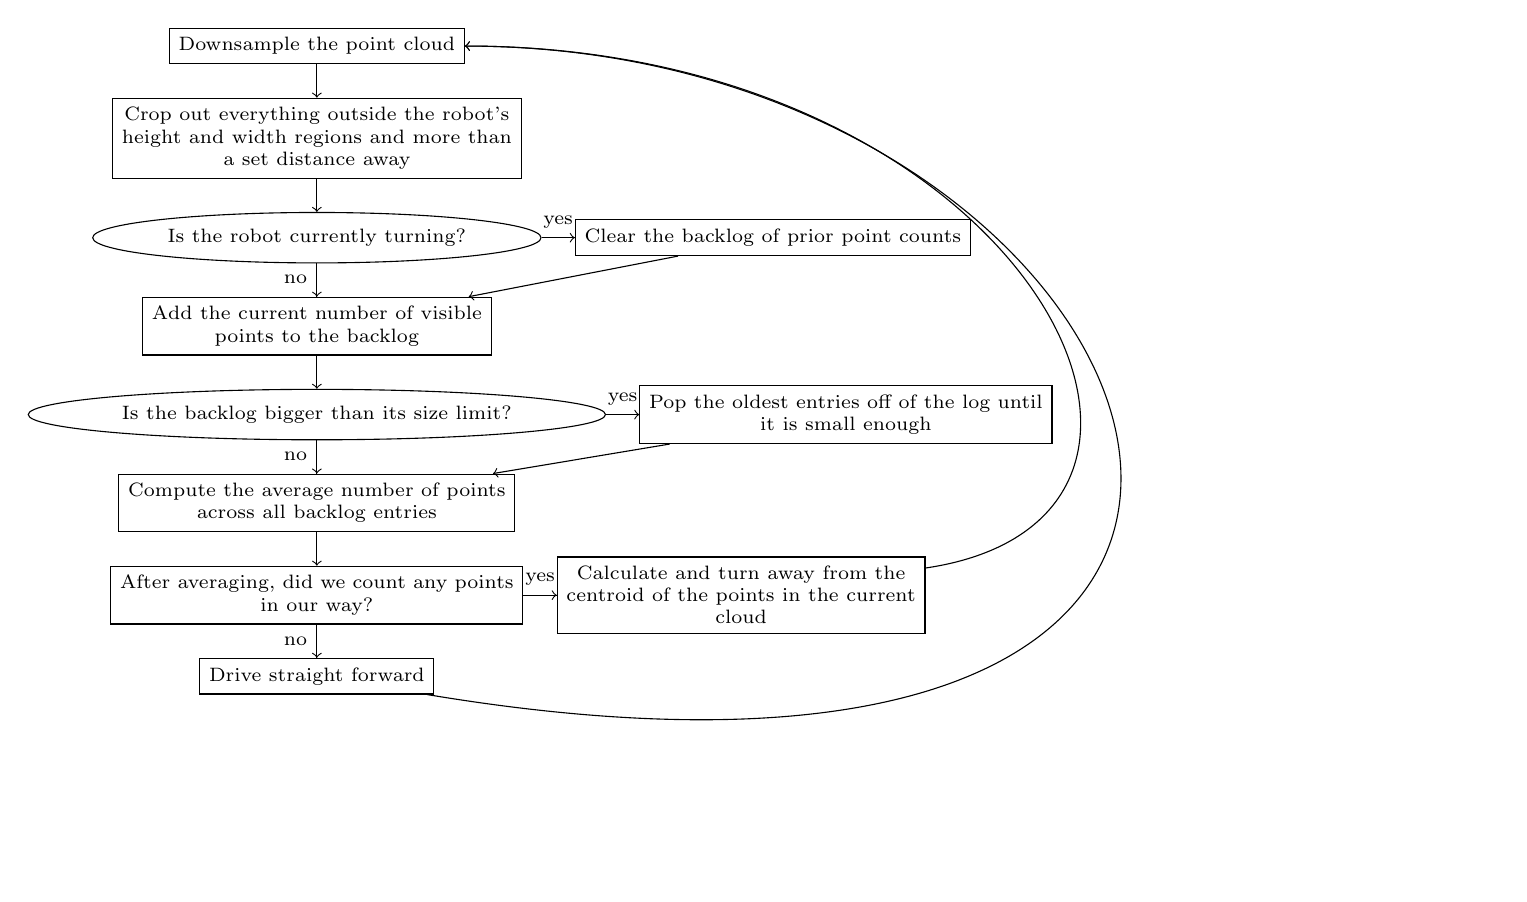
\begin{tikzpicture}[formatting/.style={font=\scriptsize,execute at begin node={\begin{varwidth}{5cm}\begin{center}},execute at end node={\end{center}\end{varwidth}}}, every node/.style={draw,on chain,formatting}, every on chain/.style=join, every join/.style=->, node distance=12pt]
{ [start chain=going below]
	\node{Downsample the point cloud};
	\node{Crop out everything outside the robot's height and width regions and more than a set distance away};
	\node[shape=ellipse]{Is the robot currently turning?};
	{ [start branch=clearlog going right]
		\node{Clear the backlog of prior point counts};
		{ [every node/.style=formatting]
			\path(chain-end) edge node[above]{yes} (chain/clearlog-end);
		}
	}
	\node[join=with chain/clearlog-end]{Add the current number of visible points to the backlog};
	{ [every node/.style=formatting]
		\path(\tikzchainprevious) edge node[left]{no} (chain-end);
	}
	\node[shape=ellipse]{Is the backlog bigger than its size limit?};
	{ [start branch=trimlog going right]
		\node{Pop the oldest entries off of the log until it is small enough};
		{ [every node/.style=formatting]
			\path(chain-end) edge node[above]{yes} (chain/trimlog-end);
		}
	}
	\node[join=with chain/trimlog-end]{Compute the average number of points across all backlog entries};
	{ [every node/.style=formatting]
		\path(\tikzchainprevious) edge node[left]{no} (chain-end);
	}
	\node{After averaging, did we count any points in our way?};
	{ [start branch=straighton going right]
		\node{Calculate and turn away from the centroid of the points in the current cloud};
		{ [every node/.style=formatting]
			\path(chain-end) edge node[above]{yes} (chain/straighton-end);
		}
		\draw[->](chain/straighton-end) .. controls (12cm,-6cm) and (9cm,0) .. (chain-1);
	}
	\node{Drive straight forward};
	{ [every node/.style=formatting]
		\path(\tikzchainprevious) edge node[left]{no} (chain-end);
	}
	\draw[->](chain-end) .. controls (15cm,-10.5cm) and (11cm,0) .. (chain-1);
}
\end{tikzpicture}
\caption{The thread performing height and width range point counting}
\label{fig:range}
\end{subfigure}
\caption{The final program's flow of control (continued on \autopageref{fig:runtimecont})}
\label{fig:runtime}
\end{figure}
\begin{figure}
\ContinuedFloat
\begin{subfigure}{\textwidth}
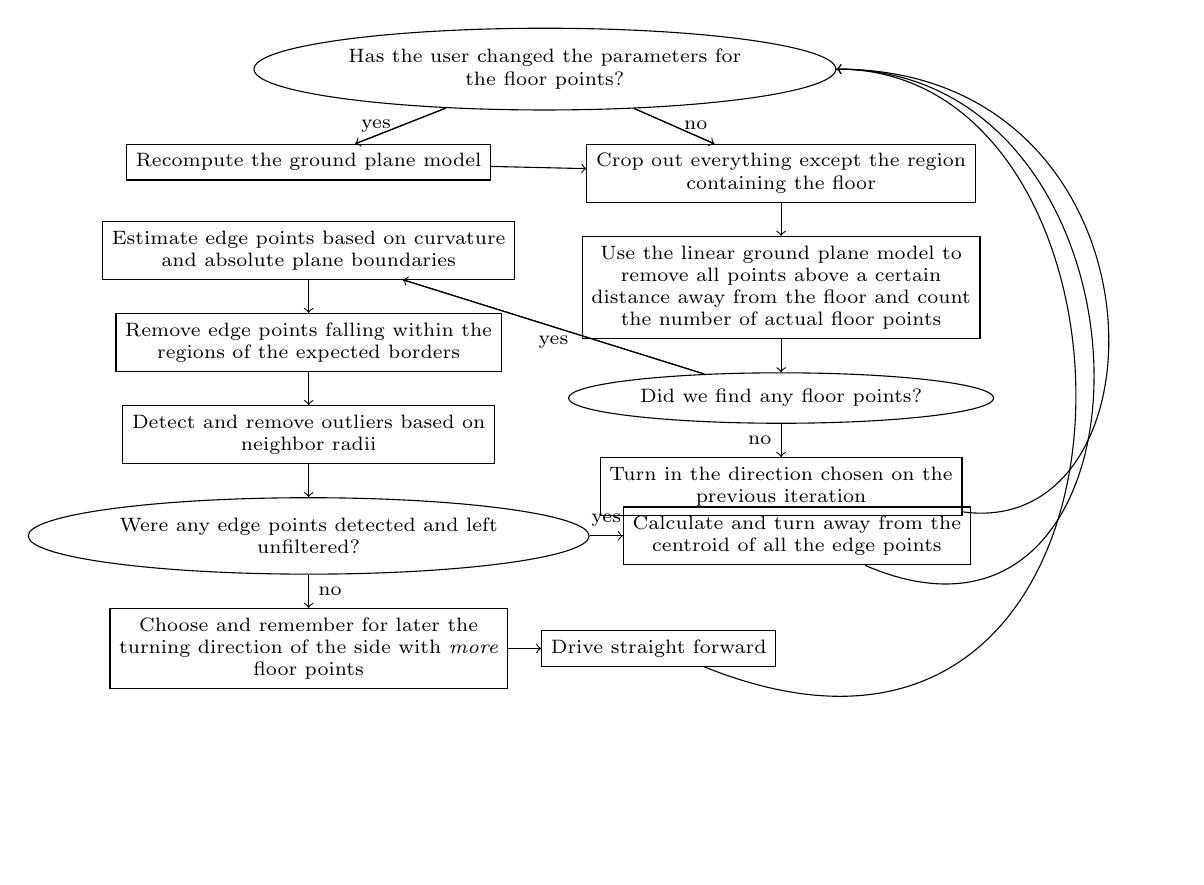
\begin{tikzpicture}[formatting/.style={font=\scriptsize,execute at begin node={\begin{varwidth}{5cm}\begin{center}},execute at end node={\end{center}\end{varwidth}}}, every node/.style={draw,on chain,formatting}, every on chain/.style=join, every join/.style=->, node distance=12pt]
{ [start chain=going below]
	\node[shape=ellipse]{Has the user changed the parameters for the floor points?};
	{ [start branch=planechanged going below]
		\node[xshift=-3cm]{Recompute the ground plane model};
		{ [every node/.style=formatting]
			\path(chain-end) edge node[left]{yes} (chain/planechanged-end);
		}
	}
	\node[join=with chain/planechanged-end,xshift=3cm]{Crop out everything except the region containing the floor};
	{ [every node/.style=formatting]
		\path(\tikzchainprevious) edge node[right]{no} (chain-end);
	}
	\node{Use the linear ground plane model to remove all points above a certain distance away from the floor and count the number of actual floor points};
	\node[shape=ellipse]{Did we find any floor points?};
	{ [start branch=floorvisible going below]
		\node[xshift=-6cm,yshift=3cm]{Estimate edge points based on curvature and absolute plane boundaries};
		{ [every node/.style=formatting]
			\path(chain-end) edge node[below]{yes} (chain/floorvisible-end);
		}
		\node{Remove edge points falling within the regions of the expected borders};
		\node{Detect and remove outliers based on neighbor radii};
		\node[shape=ellipse]{Were any edge points detected and left unfiltered?};
		{ [start branch=edgepoints going right]
			\node{Calculate and turn away from the centroid of all the edge points};
			{ [every node/.style=formatting]
				\path(chain/floorvisible-end) edge node[above]{yes} (chain/floorvisible/edgepoints-end);
			}
			\draw[->](chain/floorvisible/edgepoints-end) .. controls (8cm,-8cm) and (8cm,0) .. (chain-1);
		}
		\node{Choose and remember for later the turning direction of the side with \textit{more} floor points};
		{ [every node/.style=formatting]
			\path(\tikzchainprevious) edge node[right]{no} (chain/floorvisible-end);
		}
		\node[on chain=going right]{Drive straight forward};
		\draw[->](chain/floorvisible-end) .. controls (8cm,-10cm) and (8cm,0) .. (chain-1);
	}
	\node{Turn in the direction chosen on the previous iteration};
	{ [every node/.style=formatting]
		\path(\tikzchainprevious) edge node[left]{no} (chain-end);
	}
	\draw[->](chain-end) .. controls (8cm,-6cm) and (8cm,0) .. (chain-1);
}
\end{tikzpicture}
\caption{The thread performing surface curvature, occlusion, and visibility detection}
\label{fig:edges}
\end{subfigure}
\begin{subfigure}{\textwidth}
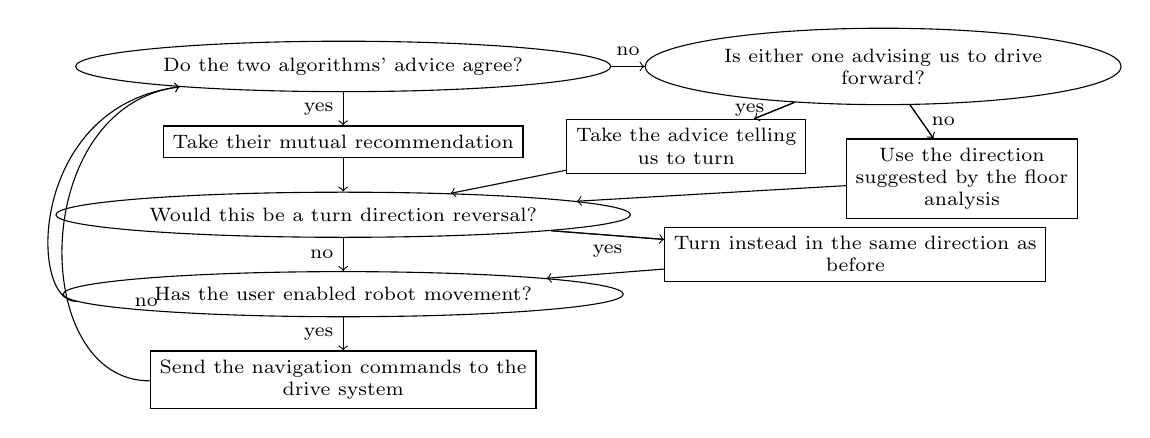
\begin{tikzpicture}[formatting/.style={font=\scriptsize,execute at begin node={\begin{varwidth}{5cm}\begin{center}},execute at end node={\end{center}\end{varwidth}}}, every node/.style={draw,on chain,formatting}, every on chain/.style=join, every join/.style=->, node distance=12pt]
{ [start chain=going below]
	\node[shape=ellipse]{Do the two algorithms' advice agree?};
	{ [start branch=atodds going right]
		\node[shape=ellipse]{Is either one advising us to drive forward?};
		{ [every node/.style=formatting]
			\path(chain-end) edge node[above]{no} (chain/atodds-end);
		}
		{ [start branch=bothturning going below]
			\node[xshift=1cm]{\begin{varwidth}{3cm}\begin{center}Use the direction suggested by the floor analysis\end{center}\end{varwidth}};
			{ [every node/.style=formatting]
				\path(chain/atodds-end) edge node[right]{no} (chain/atodds/bothturning-end);
			}
		}
		\node[on chain=going below,xshift=-2.5cm,yshift=0.25cm]{\begin{varwidth}{3cm}\begin{center}Take the advice telling us to turn\end{center}\end{varwidth}};
		{ [every node/.style=formatting]
			\path(\tikzchainprevious) edge node[left]{yes} (chain/atodds-end);
		}
	}
	\node{Take their mutual recommendation};
	{ [every node/.style=formatting]
		\path(\tikzchainprevious) edge node[left]{yes} (chain-end);
	}
	\node[shape=ellipse,join=with chain/atodds-end,join=with chain/atodds/bothturning-end]{Would this be a turn direction reversal?};
	{ [start branch=preventoscillation going right]
		\node[yshift=-0.5cm]{Turn instead in the same direction as before};
		{ [every node/.style=formatting]
			\path(chain-end) edge node[below]{yes} (chain/preventoscillation-end);
		}
	}
	\node[shape=ellipse,join=with chain/preventoscillation-end]{Has the user enabled robot movement?};
	{ [every node/.style=formatting]
		\path(\tikzchainprevious) edge node[left]{no} (chain-end);
	}
	{ [start branch=gosomewhere going below]
		\node{Send the navigation commands to the drive system};
		{ [every node/.style=formatting]
			\path(chain-end) edge node[left]{yes} (chain/gosomewhere-end);
		}
	}
	\draw[->](chain-end) .. controls (-4cm,-3cm) and (-4cm,-0.5cm).. (chain-1);
	\draw[->](chain/gosomewhere-end) .. controls (-4cm,-4cm) and (-4cm,-0.5cm) .. (chain-1);
}
{ [every node/.style=formatting]
    \node[xshift=-2.5cm,yshift=-3cm]{no};
}
\end{tikzpicture}
\caption{The thread integrating the decisions of the two detection threads and issuing appropriate drive commands}
\label{fig:pilot}
\end{subfigure}
\captionsetup{list=false}
\caption{The final program's flow of control \textit{(continued)}}
\label{fig:runtimecont}
\end{figure}

\begin{table}
\caption{Test cases to which the implementation was subjected}
\label{tab:tests}
\begin{tabular}{| p{\textwidth} |}
\hline
\textbf{Test Case} \\
\hline\hline
Encounters a wide obstacle \\
\hline
Encounters a tall, thin obstacle \\
\hline
Encounters an object that falls entirely within the center region but decidedly to one side \\
\hline
Encounters a very short but well-defined object on the ground \\
\hline
Encounters a hole (such as a staircase) \\
\hline
Encounters an object closer than the visible floor region \\
\hline
Comes extremely close to a large object or precipice \\
\hline
Encounters a suspended object (bench or vending machine) \\
\hline
Encounters a patch of sunlight \\
\hline
Encounters a glass or otherwise transparent wall \\
\hline
\end{tabular}
\end{table}

\section{Results and Discussion}
While \autoref{sec:approach} discussed the changes that were made to the code as a result of the challenges cataloged in \autoref{tab:tests}, we will now discuss the behavior of the final implementation when faced with these same scenarios.

When the autonomous robot encounters a wide obstacle, it is detected by both algorithms.  Additionally, the robot is not allowed to reverse the direction of its turn, so it cannot enter an oscillatory state.  A corollary to this behavior is that, if the robot is surrounded on all sides, it will continue spinning until freed.

Tall, thin obstacles with a limited base footprint such as a pen are best detected by the height range algorithm.  It is only thanks to the noise reduction attained by averaging several samples that it is able to spot such small objects.

In the case where an average obstacle appears in one side of the area of interest in front of the robot, it is detected by both algorithms.  Since the final revision of the cropping and downsampling approach decides directions based on the centroid of the points within the interest region, both approaches will advise turning in the same direction: away from the obstacle.

Short objects resting on the floor, including markers and pads of paper, are typically invisible to the cropping algorithm.  However, the curvature of the contact points between their edges and the ground plane is reliably detected by the other approach.

When a hole in the ground such as a descending staircase comes into view, the ground plane algorithm detects that the ground's absolute plane boundary has receded into an unexpected region.  All plane boundary points falling outside of the expected regions are treated identically to curvature points, and the direction recommendation is accordingly based on their centroid.

When an object of more than trivial height comes closer to the robot than the Kinect's point cloud is able to detect, it still distorts the emitted infrared grid so as to cast a ``shadow'' on the ground behind it.  The plane algorithm registers that the absolute plane boundary is infringing upon the center plane region, and the situation is treated in the same manner as the case of an approaching pit.

In case the robot comes close enough to an object that the Kinect's view is completely blocked, the ground plane algorithm is able to detect that it has been blinded by the complete disappearance of the floor plane.  In such a case, the robot is ordered to turn in the direction that was computed and stored when last the ground was visible.

Upon approaching a suspended or apparently-suspended object such as a bench or vending machine, the plane detection algorithm sees no change in the floor plane.  The cropping method, however, is able to see that an object is infringing upon the robot's height range, and directs it to turn away from the obstruction's centroid.

On the whole, the algorithms suffer from almost no problems with false positives.  However, the Kinect's infrared grid projection is masked by intense external infrared radiation.  If, for instance, the robot is approaching a patch of direct sunlight shining through a window, it will appear from the Kinect's point cloud as though there is a hole in the ground; the absolute plane boundary will begin to recede into the expected ground region.  Consequently, the robot will avoid such regions, treating them as actual danger.

When face-to-face with an entirely transparent glass wall, the Kinect's infrared grid passes straight through the window.  Therefore, the barrier isn't reflected in the returned point cloud, and neither algorithm is able to see it at all.

The addition of the ground plane edge detection to the traditional obstacle avoidance solution brings several key advantages:  First, examining the curvature of the plane enables the detection of almost any obstacle that makes contact with the floor, including those that are very short.  Next, looking for absolute plane edges means hazards that have no corresponding obstacle within the robot's height range---such as holes in the ground---can be easily avoided.  Finally, since objects passing in front of the infrared emitter occlude the floor in front of the sensor, examining plane edges also reveals the presence of objects suddenly appearing very close to the sensor, including animate objects whose motion is perpendicular to the robot's; in this way, the algorithm is able to infer the presence of objects that are closer than the Kinect's hardware-limited minimum range.  The latter principle makes the plane analysis approach especially beneficial for sensors such as the Kinect that are unable to see objects closer than a certain distance away.

As noted above, the complete implementation fails to perform in two of the test cases from \autoref{tab:tests}:  It is vulnerable to false positives in patches of direct sunlight and to false negatives in the case of transparent walls.  Such problems stem from the limitations of the infrared-based Kinect point cloud; however, they could likely be solved by examining the Kinect's RGB data in tandem with its depth values.

\section{Table of Hours Worked}
The time spent working on the project is addressed in \autoref{tab:hours}.  The time frame of the code's evolution is described in \autoref{fig:progression}.
\begin{table}
\caption{Hours spent working on the project}
\label{tab:hours}
\begin{tabular}{| r | r | r | r | r | r | r |}
\hline
\scriptsize\textbf{Week} & \scriptsize\textbf{Research} & \scriptsize\textbf{Implementation} & \scriptsize\textbf{Testing} & \scriptsize\textbf{Documentation} & \scriptsize\textbf{Administration} & \scriptsize\textbf{Subtotal} \\
\hline\hline
1 & 14:00 &  &  & 6:20 & 18:00 & 38:20 \\
\hline
2 & 22:00 & 9:00 & 3:00 & 3:20 & 1:30 & 38:50 \\
\hline
3 &  & 12:00 & 4:00 & 16:00 & 12:40 & 44:40 \\
\hline
4 & 3:00 & 8:00 & 5:30 & 4:00 & 5:00 & 25:30 \\
\hline
5 & 3:00 & 13:00 & 3:00 & 10:00 & 3:00 & 32:00 \\
\hline
6 &  & 9:20 & 7:00 & 3:00 & 16:20 & 35:40 \\
\hline
7 &  & 18:00 & 8:00 & 5:00 & 14:00 & 45:00 \\
\hline
8 &  & 8:00 & 5:00 & 21:00 & 8:10 & 42:10 \\
\hline
9 &  &  &  &  &  & \\
\hline\hline
&&&&& \scriptsize\textbf{Total:} & \\
\hline
\end{tabular}
\end{table}

\section{Conclusion}
The combination of the two methods of achieving obstacle avoidance was highly successful because they complemented each other so well:  The cropping approach, which was by nature incapable of detecting very short objects or floor discontinuities, was able to rely on the less common plane surface analysis for these tasks.  The plane analysis, on the other hand, was poor at detecting the truly- or apparently-suspended objects that were readily detected by the other.  As might be expected, then, the synthesis of the two algorithms was able to autonomously navigate in almost all tested indoor situations without a problem.  Thus, the project's goals were realized.

\clearpage
\phantomsection
\addcontentsline{toc}{section}{References}
{\large References} \\
\linebreak
\phantomsection
\label{bib:canny}
Canny, John. (1986). A computational approach to edge detection. In \textit{IEEE Transactions on Pattern Analysis and Machine Intelligence (PAMI),} Vol. 8, no. 6, November 1986. July 26, 2012. $\langle$\url{http://ieeexplore.ieee.org/xpl/articleDetails.jsp?arnumber=4767851}$\rangle$.

\phantomsection
\label{bib:choi}
Choi, Changhyun. (2012). Organized Edge Detection. PCL Google Summer of Code Developers Blog. July 26, 2012. $\langle$\url{http://pointclouds.org/blog/gsoc12/cchoi}

\phantomsection
\label{bib:herrera}
Herrera, Daniel \textit{et al.} (2011). Accurate and practical calibration of a depth and color camera pair. In \textit{Computer Vision, Image Analysis, and Processing (CAIP 2011).} June 8, 2012. $\langle$\url{http://www.ee.oulu.fi/~dherrera/papers/2011-depth_calibration.pdf}$\rangle$.

\phantomsection
\label{bib:holz}
Holz, Dirk \textit{et al.} (2011). Real-time plane segmentation using RGB-D cameras. In \textit{Proceedings of the 15\textsuperscript{th} RoboCup International Symposium,} Istanbul, July 2011. June 11, 2012. $\langle$\url{ais.uni-bonn.de/papers/robocup2011_holz.pdf}$\rangle$.

\phantomsection
\label{bib:koren}
Koren, Y. and Borenstein, J. (1991). Potential field methods and their inherent limitations for mobile robot navigation. In \textit{Proceedings of the IEEE Conference on Robotics and Automation,} Sacramento, April 7-12, 1991, 1398-1404. June 8, 2012. $\langle$\url{http://www-personal.umich.edu/~johannb/Papers/paper27.pdf}$\rangle$.

\begin{sloppypar}
\phantomsection
\label{bib:nguyen}
Nguyen, Van-Duc. (2012). Obstacle avoidance using the Kinect. June 15, 2012 $\langle$\url{http://scribd.com/doc/80464002/Obstacle-Avoidance-Using-the-Kinect}$\rangle$.
\end{sloppypar}

\phantomsection
\label{bib:oleary}
O'Leary, Gabe. (2011). Removing Outliers Using a Conditional or RadiusOutler Removal. Point Cloud Library Tutorials. July 26, 2012. $\langle$\url{http://pointclouds.org/documentation/tutorials/remove_outliers.php}$\rangle$.

\phantomsection
\label{bib:rusu}
Rusu, Radu B. (2011). Downsampling a PointCloud using a VoxelGrid filter. Point Cloud Library Tutorials. July 26, 2012. $\langle$\url{http://pointclouds.org/documentation/tutorials/voxel_grid.php}$\rangle$.

\phantomsection
\label{bib:talukder}
Talukder, A. \textit{et al.} (2002). Fast and reliable obstacle detection and segmentation for cross-country navigation. In \textit{Proceedings of the IEEE Intelligent Vehicle Symposium (IVS 02),} 610-618. June 25, 2012. $\langle$\url{http://users.soe.ucsc.edu/~manduchi/papers/IV02.pdf}$\rangle$.

\phantomsection
\label{bib:viola}
Viola, Paul and Jones, Michael. (2001). Robost real-time object detection. In \textit{Second International Workshop on Statistical and Computational Theories of Vision (IJCV 2001),} Vancouver, July 13, 2001. July 26, 2012. $\langle$\url{http://research.microsoft.com/~viola/Pubs/Detect/violaJones_IJCV.pdf}$\rangle$.

\clearpage
{\Large Appendices} \\
\appendix
\section{Starting the TurtleBot}
\begin{sloppypar}
\begin{enumerate}
\item{Disconnect both chargers from the robot, if applicable.}
\item{Turn on the iRobot Create by pressing the power button on its back; the power light should turn green.}
\item{Unplug and remove the laptop from the TurtleBot.}
\item{Open the laptop's lid and press the power button.}
\item{Close the laptop, replace it in the chassis, and reconnect the cables.}
\item{Wait until the Ubuntu startup noise sounds; at this point, the robot is ready to accept connections.}
\item{From another machine, enter: \texttt{\$\ ssh turtlebot@turtlebot.rit.edu}}
\item{Once authenticated, ensure that the robot service is running: \texttt{\$\ sudo service turtlebot start}}
\item{The iRobot Create should beep and its power light should go out.  The robot is now ready for use.}
\item{Enter the following command to enable the Kinect: \texttt{\$\ nohup roslaunch turtlebot\_bringup kinect.launch \&}}
\item{Enter the following command to enable the Interactive tab in RViz and allow GUI-driven teleoperation: \texttt{\$\ nohup rosrun turtlebot\_interactive\_markers turtlebot\_marker\_server \&}}
\item{You may now safely close your robot shell connection: \texttt{\$\ exit}}
\end{enumerate}
\end{sloppypar}

\section{Stopping the TurtleBot}
\begin{sloppypar}
\begin{enumerate}
\item{Connect to the robot.}
\item{Stop the Interactive Markers server: \texttt{\$\ kill `ps -ef | grep marker\_server | tr -s " " | cut -d " " -f 2`}}
\item{Stop the Kinect driver with: \texttt{\$\ kill `ps -ef | grep kinect.launch | grep -v grep | tr -s " " | cut -d " " -f 2`}}
\item{Release the iRobot Create with: \texttt{\$\ rosservice call /turtlebot\_node/set\_operation\_mode 1}}
\item{At this point, it is safe to plug the charger into the iRobot Create.  If you want to turn off the laptop as well, continue with the below steps instead.}
\item{Shut down the robot laptop: \texttt{\$\ sudo halt}}
\item{Turn off the Create by pressing its power button.}
\item{Plug in the chargers for the iRobot Create and the laptop.}
\end{enumerate}
\end{sloppypar}

\section{Setting up a Development Workstation}
\begin{sloppypar}
\begin{enumerate}
\item{Ready a machine for your use.  (We'll assume you're using Ubuntu 10.04 through 11.10.)}
\item{Ensure that your system has either a hostname or a static IP that is visible from the robot.}
\item{Download the ROS package signing key: \texttt{\$\ wget http://packages.ros.org/ros.key}}
\item{Add the signing key to your system: \texttt{\$\ sudo apt-key add ros.key}}
\item{Add the ROS repository to your system: \texttt{\$\ sudo apt-add-repository http://packages.ros.org/ros/ubuntu}}
\item{Update your repository cache: \texttt{\$\ sudo apt-get update}}
\item{Install the TurtleBot desktop suite: \texttt{\$\ sudo apt-get install ros-electric-turtlebot-desktop}}
\item{Edit your bash configuration(\texttt{\$\ \$EDITOR \~{}/.bashrc}), adding the following lines to the end:}
\begin{alltt}
\begin{itemize}
\item{}
\item{source /opt/ros/electric/setup.bash}
\item{export ROS\_MASTER\_URI=http://turtlebot.rit.edu:11311}
\item{export ROS\_PACKAGE\_PATH=<directory\- where\- you'll\- store\- your\- source\- code>:\$ROS\_PACKAGE\_PATH}
\end{itemize}
\end{alltt}
\item{Write and close the file, then enter the following command in each of your open terminals: \texttt{\$\ source \~{}/.bashrc}}
\item{Install the Chrony NTP daemon: \texttt{\$\ sudo apt-get install chrony}}
\item{Synchronize the clock: \texttt{\$\ sudo ntpdate ntp.rit.edu}}
\item{If the robot and the workstation both have hostnames, but they are in different domains, perform the following steps.  (In this example, the robot is at \texttt{turtlebot.rit.edu} and the workstation is at \texttt{turtlecmd.wireless.rit.edu}.)}
\begin{enumerate}
\item{On each machine, right-click the Network Manager applet in the notification area, choose \textit{Edit Connections...}, and open the properties for the specific connection that is being used.}
\item{On the IPv4 Settings tab, change the \textit{Method} dropdown to \texttt{Automatic (DHCP) address only.}}
\item{In the \textit{DNS servers} field, enter the same DNS servers that were being used, with commas in between (e.g. \texttt{129.21.3.17, 129.21.4.18}).}
\item{In the \textit{Search domains} field, enter the local machine's domain first, followed by the remote machine's.  For instance, in our example, one might enter \texttt{rit.edu., wireless.rit.edu.} on the robot and \texttt{wireless.rit.edu., rit.edu.} on the workstation.}
\item{Save all your changes and exit the Network Connections dialog.}
\item{Force a reconnection by clicking on the Network Manager applet, then selecting the network to which you are already connected.}
\end{enumerate}
\item{If the workstation has no qualified hostname and is to be reached via a static IP, make the following changes on the robot instead:}
\begin{enumerate}
\item{Edit the robot's hosts file: \texttt{\$\ sudo \$EDITOR /etc/hosts}}
\item{For each static host, add a line such as: \texttt{$\langle$IP address$\rangle$ $\langle$hostname$\rangle$}.  It is important to note that the \textit{hostname} you use must exactly match the output of \texttt{\$\ hostname} on the development workstation.}
\item{Save the file and quit; the changes should take effect immediately and automatically.}
\end{enumerate}
\end{enumerate}
\end{sloppypar}

\section{Upgrading to the Latest Version of PCL}
\label{apx:upgrade}
The version of the Point Cloud Library shipped with ROS lags significantly behind that available directly from the community.  These instructions show how to install the latest version of PCL on top of an existing ROS Electric installation.
\begin{sloppypar}
\begin{enumerate}
\item{Create a folder to contain the build files and a replacement copy of the \texttt{perception\_pcl} stack: \texttt{\$\ mkdir \~{}/ros}}
\item{Install the Python package management utilities: \texttt{\$\ sudo apt-get install python-setuptools}}
\item{Install the dependencies for the \texttt{rosinstall} utility: \texttt{\$\ sudo easy\_install -U rosinstall}}
\item{Create a new ROS overlay in the current directory: \texttt{\$\ rosinstall . /opt/ros/electric}}
\item{Install any missing build dependencies: \texttt{\$\ rosdep install perception\_pcl}}
\item{Obtain a rosinstall file describing the repository for the perception stack: \texttt{\$\ roslocate info perception\_pcl $\rangle$ perception\_pcl.rosinstall}}
\item{Edit the rosinstall file to point at the correct repository for Electric: \texttt{\$\ sed -i s/unstable/electric\_unstable/ perception\_pcl.rosinstall }}
\item{Fetch the makefiles for the stack: \texttt{\$\ rosinstall . perception\_pcl.rosinstall}}
\item{Inform your shell of the overlay's location: \texttt{\$\ source setup.bash}}
\item{Move into the \texttt{cminpack} directory: \texttt{\$\ cd perception\_pcl/cminpack}}
\item{Build the package: \texttt{\$\ make}}
\item{Move into the \texttt{flann} directory: \texttt{\$\ cd ../flann}}
\item{Build the package: \texttt{\$\ make}}
\item{Move into the \texttt{pcl} directory: \texttt{\$\ cd ../pcl}}
\item{Make a backup copy of the makefile: \texttt{\$\ cp Makefile Makefile.orig}}
\item{Select the most recent tagged version of the code, for instance: \texttt{\$\ sed -i s/$\backslash\backslash$/trunk/$\backslash\backslash$/tags$\backslash\backslash$/pcl-1.6.0/ Makefile}}
\item{Build the PCL codebase: \texttt{\$\ make}}
\item{Move into the \texttt{pcl\_ros} directory: \texttt{\$\ cd ../pcl\_ros}}
\item{Build the ROS PCL bindings: \texttt{\$\ make}}
\item{Move back out into the stack: \texttt{\$\ cd ..}}
\item{Build the stack's particulars: \texttt{\$\ make}}
\item{Edit your \texttt{bashrc} file to add the following line after the line that sources the system-wide ROS \texttt{setup.bash}: \texttt{source \~{}/ros/setup.bash}}
\item{If you intend on continuing to use your current terminals, enter the following in each after saving the file: \texttt{\$\ source \~{}/.bashrc}}
\end{enumerate}
\end{sloppypar}

\section{Backporting in a Class from the PCL Trunk}
Often, the trunk version of the Point Cloud Library will fail to compile; therefore, it may be desirable to backport a specific class from trunk into a released copy of the library.  For instance, the code written for this project relies on the OrganizedEdgeDetection class, which---at the time of writing---is only available from trunk.  These steps present an example of how to backport this specific class and the new subsystem on which it relies into the 1.6.0 release of PCL.  We'll assume that the steps from \autoref{apx:upgrade} of the Appendix have already been completed.
\begin{sloppypar}
\begin{enumerate}
\item{Change to the directory above your newly-compiled copy of the Point Cloud Library: \texttt{\$\ roscd pcl/..}}
\item{Make a copy of the whole library folder: \texttt{\$\ cp -r pcl pcl.trunk}}
\item{Move into the folder you just created: \texttt{\$\ cd pcl.trunk}}
\item{Restore the backup version of the makefile in order to switch back to trunk: \texttt{\$\ mv Makefile.orig Makefile}}
\item{Clean out the directory: \texttt{\$\ make wipe}}
\item{Re-download the latest code: \texttt{\$\ make download}}
\item{Move back up one level in preparation for copying over the new files: \texttt{\$\ cd ..}}
\item{Copy the header from trunk to release: \texttt{\$\ cp pcl.trunk\slash build\slash pcl\_trunk\slash features\slash include\slash pcl\slash features\slash organized\_edge\_detection.h pcl\slash build\slash pcl\_trunk\slash features\slash include\slash pcl\slash\slash features}}
\item{Copy the templated header from trunk to release: \texttt{\$\ cp pcl.trunk\slash build\slash pcl\_trunk\slash features\slash include\slash pcl\slash features\slash impl\slash organized\_edge\_detection.hpp pcl\slash build\slash pcl\_trunk\slash features\slash include\slash pcl\slash features\slash impl}}
\item{Copy the source from trunk to release: \texttt{\$\ cp pcl.trunk\slash build\slash pcl\_trunk\slash features\slash src\slash organized\_edge\_detection.cpp pcl\slash build\slash pcl\_trunk\slash features\slash src}}
\item{Copy a required new subsystem from trunk to release: \texttt{\$\ cp -r pcl.trunk/build/pcl\_trunk/2d pcl/build/pcl\_trunk}}
\item{Move into the newly-assembled PCL build directory: \texttt{\$\ cd pcl/build/pcl\_trunk}}
\item{Edit the \texttt{2d} package's build configuration file: \texttt{\$\ \$EDITOR 2d/CMakeLists.txt}}
\begin{enumerate}
\item{For each header linked under \texttt{set(incs}, check whether it has a templated header in \texttt{2d/include/pcl/2d/impl}.}
\item{For each such header, add a corresponding line under \texttt{set(impl\_incs}; for instance, the line to add for \texttt{include/pcl/\$\{SUBSYS\_NAME\}/convolution\_2d.h} would be \texttt{include/pcl/\$\{SUBSYS\_NAME\}/impl/convolution\_2d.hpp}}
\end{enumerate}
\item{Edit the \texttt{features} package's build configuration: \texttt{\$\ \$EDITOR features/CMakeLists.txt}}
\begin{enumerate}
\item{At the end of the SUBSYS\_DEPS list, add: \texttt{2d}}
\item{Under \texttt{set(incs}, add: \texttt{include\slash pcl\slash \$\{SUBSYS\_NAME\}\slash organized\_edge\_detection.h}}
\item{Under \texttt{set(impl\_incs}, add: \texttt{include\slash pcl\slash \$\{SUBSYS\_NAME\}\slash impl\slash organized\_edge\_detection.hpp}}
\item{Under \texttt{set(srcs}, add: \texttt{src/organized\_edge\_detection.cpp}}
\end{enumerate}
\item{Apply any custom patches to the code as required.}
\item{Return to the package root: \texttt{\$\ roscd pcl}}
\item{Mark the package as needing to be rebuilt: \texttt{\$\ rm installed}}
\item{Build in the changes and relink: \texttt{\$\ make}}
\end{enumerate}
\end{sloppypar}

\section{ROS Glossary}
\begin{itemize}
\begin{sloppypar}
\item{\textbf{message.} A ROS communication packet that carries information between \textit{nodes} in a single direction.  New message types may be declared by creating text files in a package's \texttt{msg} directory and enabling the \texttt{rosbuild\_genmsg()} directive in its \texttt{CMakeLists.txt} file.  The composition of existing message types may be found using the \texttt{rosmsg show} command.  ROS automatically generates a C++ struct for each message type; these struct types are declared in the \texttt{$\langle$package$\rangle$/$\langle$messagetype$\rangle$.h} headers; these must be included before they may be used.  Two examples of useful message types are \texttt{std\_msgs/Int32}---an \texttt{int}---and \texttt{geometry\_msgs/Twist}---used for driving the Create around.}
\item{\textbf{node.} A single ROS executable, which may be added to a \textit{package} by appending a \texttt{rosbuild\_add\_executable} directive to the \texttt{CMakeLists.txt} file of the latter.  Once the package has been compiled using GNU Make, each of its nodes may be run using the \texttt{rosrun} command.}
\end{sloppypar}
\item{\textbf{package.} A ``project'' containing executables and/or libraries; new packages may be created with the \texttt{roscreate-pkg} command, and existing ones may be imported into a dependent one by adding \texttt{depend} tags to its \texttt{manifest.xml} file.  A couple of important packages are \texttt{roscpp}, which contains the \texttt{ros/ros.h} header that allows one to interface with ROS, and \texttt{pcl\_ros}, which depends on the \texttt{pcl} package to provide the Point Cloud Library bindings.}
\item{\textbf{parameter.} A variable hosted on the ROS parameter server; it is persistent across multiple runs of a node, provided that the ROS master is not restarted.  Depending upon the node's implementation, changing one of its parameters while it is running may also affect its continued behavior.  The user interface to the parameter server is provided by the \texttt{rosparam} command, while the C++ API supports the analogous \texttt{setParam}, \texttt{getParam}, \texttt{deleteParam}, and other methods located in the \texttt{ros::NodeHandle} class.}
\begin{sloppypar}
\item{\textbf{service.} A link between ROS \textit{nodes} allowing two-way communication carried in the form of service types from a client to a server.  The user may call an existing service using the \texttt{rosservice} command, while C++ programs may create and call services via the \texttt{ros::ServiceServer} and \texttt{ros::ServiceClient} classes, which may be built by means of the \texttt{advertiseService} and \texttt{serviceClient} methods of \texttt{ros::NodeHandle}.  Service types---the analog of \textit{messages} from the world of \textit{topics}---may be declared in text files within a package's \texttt{srv} directory after enabling its \texttt{CMakeLists.txt} file's \texttt{rosbuild\_gensrv()} call.  Service types' components may be seen with the \texttt{rosservice show} invocation, and C++ service structs are generated and used similarly to those for \textit{messages}.  One example of a service used on the TurtleBot is \texttt{/turtlebot\_node/set\_operation\_mode}, which takes an integer---usually 1, 2, or 3---responds whether it is valid, and brings the iRobot Create into either Passive, Safety, or Full mode, respectively.}
\end{sloppypar}
\item{\textbf{topic.} A link between ROS \textit{nodes} that allows one-way communication of information carried in the form of \textit{messages} from a publisher to one or more subscribers.  The user may publish or subscribe to a topic by means of the \texttt{rostopic} command, while C++ programs may do so by creating a \texttt{ros::Publisher} or \texttt{ros::Subscriber} object using the \texttt{ros::NodeHandle} class's \texttt{advertise} or \texttt{subscribe} method.  Examples of topics on the TurtleBot are \texttt{/cmd\_vel}---modified in order to to control the Create's drive and steering---and \texttt{/cloud\_throttled}---which provides the point cloud from the Kinect.}
\end{itemize}

\section{ROS Commands}
This section aims to list the commands needed to interface with ROS and briefly address their commonly-used arguments.  For the sake of clarity, the following conventions are used: unless otherwise noted, arguments in $\langle$angled brackets$\rangle$ are required, while those in [square brackets] are optional.
\begin{itemize}
\item{\textbf{roscore} brings up a ROS master, which is useful for experimenting with ROS on one's workstation when the TurtleBot is not online.  However, in order to actually use this master instead of the TurtleBot's, one must do the following in each pertinent shell: \texttt{\$\ export ROS\_MASTER\_URI=http://localhost:11311}}
\item{\textbf{roscd $\langle$package$\rangle$} is a convenience script that allows one to immediately move into the root directory of the specified \textit{package}.}
\item{\textbf{roscreate-pkg $\langle$package$\rangle$ [dependencies]} initializes package directories to contain the source code for one or more modules.  The package directory structure will be created in a new subdirectory called \textit{package} within the current folder, which must appear in \texttt{\$ROS\_PACKAGE\_PATH}.  Typically, the \textit{dependencies} should include the \texttt{roscpp} package---which contains the ROS C++ bindings---as well as any other ROS packages that will be used, such as \texttt{pcl\_ros}.  The dependencies may be modified later by editing the \texttt{manifest.xml} file in the root directory of the package to add additional \texttt{depend} tags.  ROS nodes may be added to a project by adding a \texttt{rosbuild\_add\_executable} directive to the \texttt{CMakeLists.txt} file, also located in the package root.}
\begin{sloppypar}
\item{\textbf{rosmsg $\langle$verb$\rangle$ $\langle$arguments$\rangle$} shows information about currently-defined message types that may be passed over topics.  When \textit{verb} is \texttt{show} and the \textit{arguments} are \texttt{$\langle$package$\rangle$/$\langle$messagetype$\rangle$}, for instance, an ``API reference'' of the types and names of the variables in the message's corresponding struct hierarchy is displayed.}
\end{sloppypar}
\item{\textbf{rosparam $\langle$verb$\rangle$ $\langle$parameterpath$\rangle$} supports \textit{verb}s such as: \texttt{list}, \texttt{set}, \texttt{get}, and \texttt{delete}.  In the case of the former, the \textit{parameterpath} may be omitted if a complete listing is desired.  The \texttt{set} invocation expects an additional argument containing the new value to be appended.}
\item{\textbf{rosrun $\langle$package$\rangle$ $\langle$node$\rangle$} is simply used to execute a \textit{node} once the \textit{package} has been compiled with \texttt{make}.}
\item{\textbf{rosservice $\langle$verb$\rangle$ $\langle$servicepath$\rangle$} allows interfacing with the presently-available services over which service types may be sent.  When \textit{verb} is \texttt{list}, \textit{servicepath} may optionally be omitted, in which case all services will be shown.  With \texttt{call}, the user may call a service by passing arguments and receive a response as supported by the service type.  The \texttt{type} \textit{verb} is important, as it returns the package and service type corresponding to the service at the specified path.}
\item{\textbf{rossvc $\langle$verb$\rangle$ $\langle$arguments$\rangle$} allows querying currently-defined service types for passing over services.  When \textit{verb} is \texttt{show} and the \textit{arguments} are of the form \texttt{$\langle$package$\rangle$/$\langle$servicetype$\rangle$}, the command outputs an ``API reference''--style listing of the types and names of the variables in the struct type representing the service type.}
\item{\textbf{rostopic $\langle$verb$\rangle$ $\langle$topicpath$\rangle$} provides a bridge to currently-advertised topics over which messages may be passed.  When \textit{verb} is \texttt{list}, \textit{topicpath} may optionally be omitted to list all available topics.  With \texttt{echo}, the user may subscribe to a topic and view the data that is being subscribed to it.  Conversely, invocation with \texttt{pub} allows publishing to the topic, which will influence the nodes that are presently subscribed to it.  The \texttt{type} \textit{verb} is particularly useful: it prints the package and message type of a given registered topic.}
\end{itemize}

\section{Useful Links}
Unfortunately, much of the ROS documentation is rather terse and unfriendly.  Here, I've made an effort to catalog the documentation that I found most helpful.  I've also included documentation from the PCL website, which is perhaps better organized and certainly more comprehensive than that available on the ROS Wiki.
\begin{sloppypar}
\begin{itemize}
\item{ROS TurtleBot wiki: \url{http://ros.org/wiki/TurtleBot}}
\item{ROS tutorials: \url{http://ros.org/wiki/ROS/Tutorials}}
\item{ROS C++ tutorials: \url{http://ros.org/wiki/roscpp/Tutorials}}
\item{ROS C++ overview: \url{http://ros.org/wiki/roscpp/Overview}}
\item{ROS C++ API reference: \url{http://ros.org/doc/electric/api/roscpp/html}}
\item{ROS Kinect calibration tutorials: \url{http://ros.org/wiki/openni_launch/Tutorials}}
\item{ROS PCL data type integration examples: \url{http://ros.org/wiki/pcl_ros}}
\item{PCL tutorials: \url{http://pointclouds.org/documentation/tutorials}}
\item{PCL API reference (1.1.0): \url{http://docs.pointclouds.org/1.1.0}}
\item{PCL API reference (1.6.0): \url{http://docs.pointclouds.org/1.6.0}}
\item{PCL API reference (trunk): \url{http://docs.pointclouds.org/trunk}}
\end{itemize}
\end{sloppypar}

\end{document}
